% ============================================================================
% 20-Minute Presentation - ViT Training Strategies on ImageNette
% Author: Junjie
% Duration: 20 minutes
% ============================================================================

\documentclass[aspectratio=169]{beamer}

% Multiple theme layers
\usetheme{Boadilla}
\usetheme{CambridgeUS}
\usefonttheme{structuresmallcapsserif}
\usepackage{bookman}
\usetheme{Madrid}

% Packages
\usepackage[utf8]{inputenc}
\usepackage{graphicx}
\usepackage{booktabs}
\usepackage{amsmath}
\usepackage[absolute,overlay]{textpos}
\usepackage{pifont}
\newcommand{\cmark}{\ding{51}}  % checkmark
\newcommand{\xmark}{\ding{55}}  % x mark
\newcommand{\starmark}{\ding{72}} % star

% Final theme
\usetheme{Warsaw}
\useoutertheme{infolines}

% Show all section names in header navigation (no auto divider slides)

% Shrink all slide body text to fit
\setbeamerfont{frametitle}{size=\normalsize}
\setbeamertemplate{itemize items}[circle]
\setlength{\leftmargini}{1.2em}
\setlength{\leftmarginii}{1em}

% ============================================================================
% TITLE PAGE
% ============================================================================
\title[ViT Training Strategies]{Comparing Vision Transformer Training Strategies on ImageNette}

\author[Junjie]{\textbf{Junjie\\ \footnotesize AI Final Project}}

\institute[MSCS 2203]{\textbf{Department of Computer Science\\Artificial Intelligence Course (MSCS 2203)}}

\date{March 2026}

% ============================================================================
% DOCUMENT
% ============================================================================
\begin{document}

\begin{frame}
    \titlepage
\end{frame}

\begin{frame}
    \frametitle{Outline}
    \tableofcontents
\end{frame}

% ============================================================================
\section{Introduction}

\begin{frame}
    \frametitle{Previous Project Recap (ML, Dec 2025)}
    \small
    \begin{columns}
        \begin{column}{0.55\textwidth}
            
\includegraphics[width=\textwidth]{prev_figures/metrics_comparison.png}
        \end{column}
        \begin{column}{0.44\textwidth}
            \textbf{CNN vs ResNet on CIFAR-10:}
            \begin{itemize}
                \item[\cmark] ResNet-30 won: \textbf{94.28\%}
                \item[\cmark] 82\% fewer params than CNN
                \item[\cmark] 33\% faster convergence
            \end{itemize}
            \vspace{0.15cm}
            \textbf{Future Work identified:}
            \begin{itemize}
                \item[$\Rightarrow$] Higher-resolution datasets
                \item[$\Rightarrow$] Transfer learning
                \item[$\Rightarrow$] Attention mechanisms
            \end{itemize}
            \vspace{0.15cm}
            \begin{block}{This Project}
                Addresses \textbf{all three}!
            \end{block}
        \end{column}
    \end{columns}
\end{frame}

\begin{frame}
    \frametitle{Previous Results: Training \& Confusion Matrices}
    \begin{columns}
        \begin{column}{0.5\textwidth}
            
\includegraphics[width=\textwidth]{prev_figures/training_curves.png}
        \end{column}
        \begin{column}{0.5\textwidth}
            
\includegraphics[width=\textwidth]{prev_figures/confusion_matrices.png}
        \end{column}
    \end{columns}
    \vspace{0.15cm}
    \small
    CNNs converge well on small data (inductive bias). \textbf{New question:} \textit{How much does pretraining improve ViT?}
\end{frame}

\begin{frame}
    \frametitle{What is a Vision Transformer (ViT)?}
    \small
    \textbf{Traditional CNN:} Scans image with small filters (3$\times$3), local receptive fields

    \vspace{0.15cm}

    \textbf{Vision Transformer:} Treats image as a sequence of patches
    \begin{itemize}
        \item Split 224$\times$224 image into 196 patches (16$\times$16 each)
        \item Flatten each patch into a vector (768 dimensions)
        \item Add position embeddings (so model knows spatial layout)
        \item Process through 12 Transformer layers with \textbf{self-attention}
        \item CLS token $\rightarrow$ classification head $\rightarrow$ prediction
    \end{itemize}

    \vspace{0.15cm}

    \begin{alertblock}{Key Difference from CNNs}
        Self-attention lets every patch attend to \textbf{every other patch} simultaneously.
        No locality bias --- the model must \textit{learn} spatial relationships from data.
    \end{alertblock}
\end{frame}

\begin{frame}
    \frametitle{The Research Question}

    \begin{center}
        \Large
        \textbf{Given the same ViT-Base model (86M params),}\\[0.3cm]
        \textbf{how much does pretraining improve performance?}
    \end{center}

    \vspace{0.2cm}

    \begin{table}
        \centering
        \begin{tabular}{lll}
            \toprule
            \textbf{Strategy} & \textbf{What's Pretrained?} & \textbf{What Trains?} \\
            \midrule
            \xmark\ From Scratch & Nothing & Everything (85.8M) \\
            \cmark\ Linear Probe & Backbone (frozen) & Head only (7,690) \\
            \cmark\ Fine-Tuned & Backbone (unfrozen) & Everything (85.8M) \\
            \bottomrule
        \end{tabular}
    \end{table}

    \vspace{0.15cm}

    \begin{block}{Hypothesis}
        Pretraining will dramatically improve ViT accuracy on small datasets
    \end{block}
\end{frame}

% ============================================================================
\section{Methodology}

\begin{frame}
    \frametitle{Dataset: ImageNette}
    \small
    \begin{columns}
        \begin{column}{0.48\textwidth}
            \textbf{What is ImageNette?}
            \begin{itemize}
                \item 10 ImageNet classes, $\sim$13,400 images
                \item 224$\times$224 pixels (full resolution)
                \item Train: $\sim$9,469 | Val: $\sim$3,925
            \end{itemize}
            \vspace{0.15cm}
            \textbf{Why not CIFAR-10?}
            \begin{itemize}
                \item CIFAR-10: 32$\times$32 $\rightarrow$ only 4 patches!
                \item ImageNette: 224$\times$224 $\rightarrow$ 196 patches
                \item Real ImageNet images
            \end{itemize}
            \vspace{0.1cm}
            {\footnotesize \textbf{GPU:} NVIDIA RTX PRO 6000 Blackwell (102GB)\\
            \textbf{Total time:} $\sim$31.5 min for all 3 experiments}
        \end{column}
        \begin{column}{0.5\textwidth}
            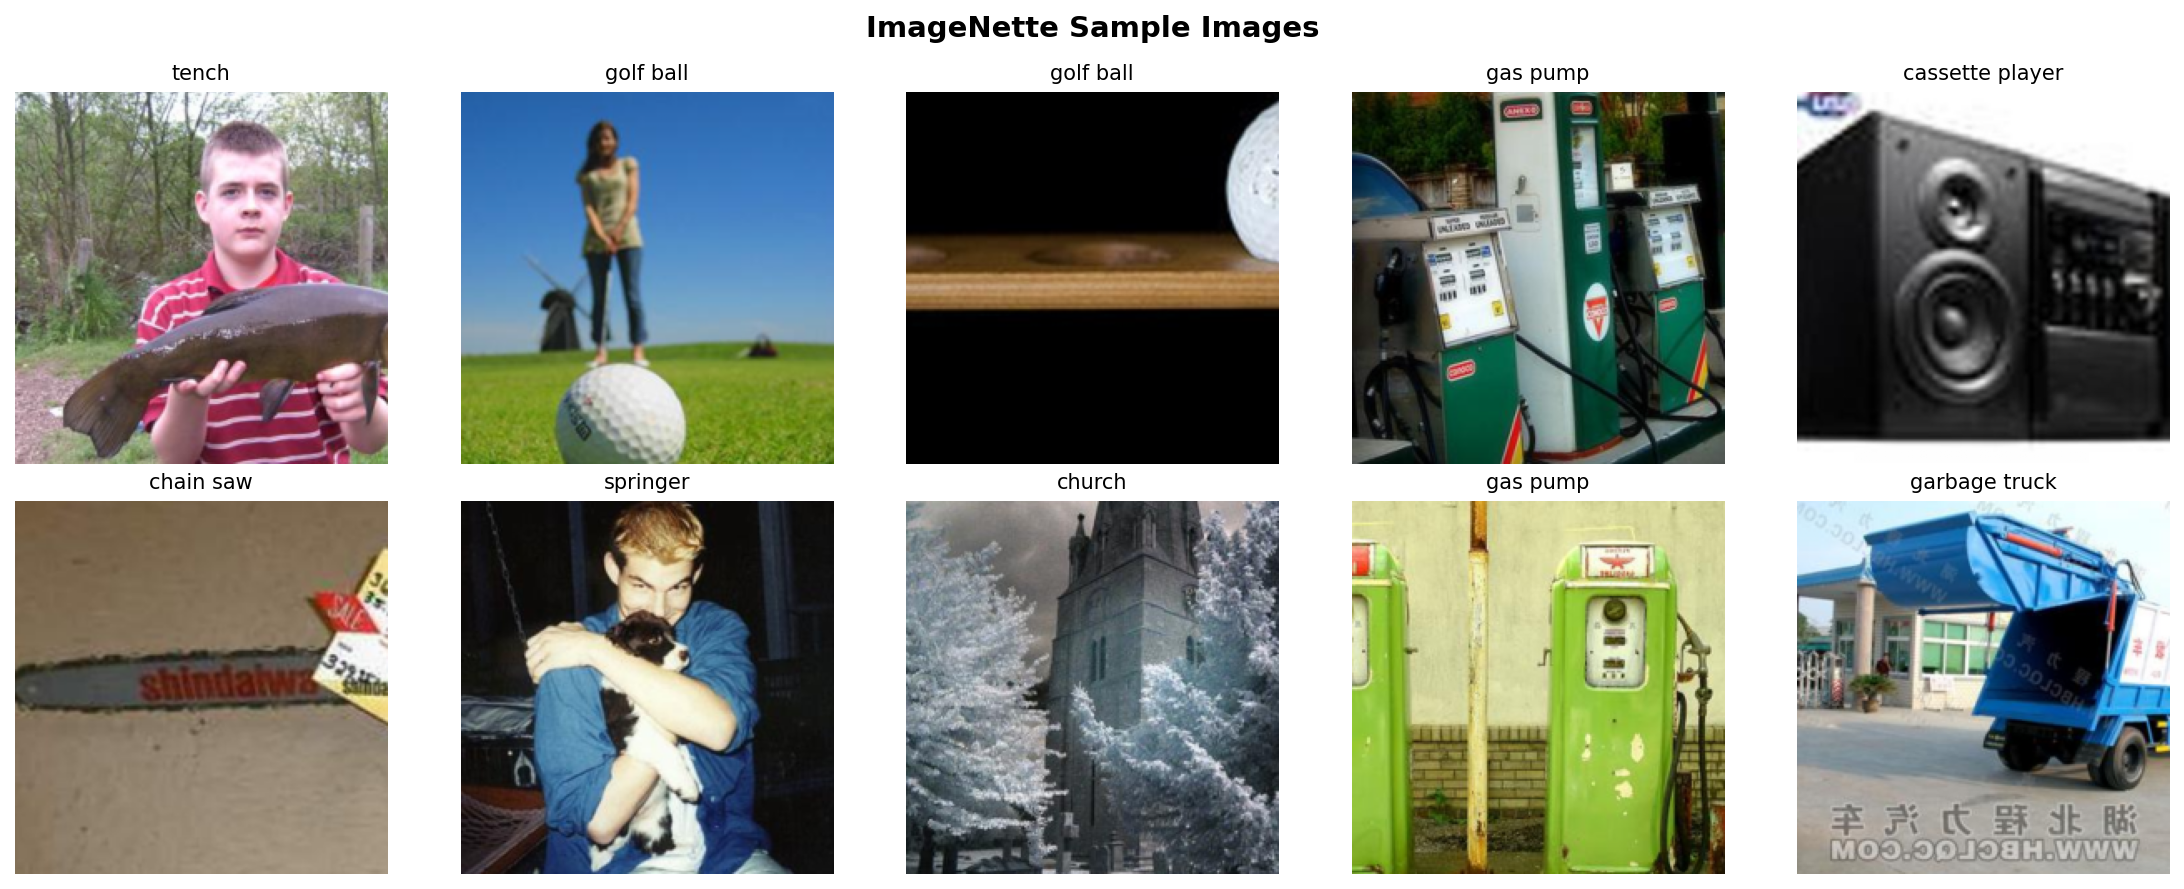
\includegraphics[width=\textwidth]{figures/sample_images.png}
        \end{column}
    \end{columns}
\end{frame}

\begin{frame}
    \frametitle{Training Configuration}
    \small
    \begin{table}
        \centering
        \begin{tabular}{lccc}
            \toprule
            & \textbf{From Scratch} & \textbf{Linear Probe} & \textbf{Fine-Tuned} \\
            \midrule
            Epochs & 50 & 20 & 10 \\
            Learning Rate & $1 \times 10^{-3}$ & $1 \times 10^{-2}$ & $2 \times 10^{-5}$ \\
            Batch Size & 64 & 128 & 32 \\
            Trainable Params & 85.8M & 7,690 & 85.8M \\
            \bottomrule
        \end{tabular}
    \end{table}

    \textbf{Shared Settings:}
    \begin{itemize}
        \item \textbf{Optimizer:} AdamW with cosine annealing + linear warmup
        \item \textbf{Augmentation:} Random crop (224), horizontal flip, normalization
        \item \textbf{Gradient clipping:} Max norm 1.0
    \end{itemize}
    {\footnotesize Same architecture, same data, same evaluation --- only strategy differs. Seed = 42.}
\end{frame}

\begin{frame}
    \frametitle{Evaluation Metrics}
    \small
    \textbf{Standard Metrics (same as previous project):}
    \begin{itemize}
        \item \textbf{Accuracy}, \textbf{Precision}, \textbf{Recall} (macro-averaged), \textbf{F1-Score}, \textbf{ROC-AUC} (one-vs-rest)
    \end{itemize}

    \vspace{0.1cm}

    \textbf{New --- ViT-Specific Analysis:}
    \begin{itemize}
        \item Attention map visualization (what does the model look at?)
        \item Multi-layer attention evolution (how attention changes across layers)
        \item Position embedding similarity (learned spatial structure)
    \end{itemize}

    \vspace{0.1cm}
    {\footnotesize \textbf{Reproducibility:} Fixed seeds, deterministic CUDA, consistent data splits.}
\end{frame}

% ============================================================================
\section{Results}

\begin{frame}
    \frametitle{Main Results - Overall Performance}

    \begin{table}
        \centering
        \Large
        \begin{tabular}{lcccc}
            \toprule
            \textbf{Strategy} & \textbf{Accuracy} & \textbf{Precision} & \textbf{Recall} & \textbf{F1} \\
            \midrule
            From Scratch & 37.30\% & 0.4526 & 0.3750 & 0.3443 \\
            \textbf{Linear Probe} & \textcolor{red}{\textbf{99.67\%}} & \textbf{0.9967} & \textbf{0.9967} & \textbf{0.9967} \\
            Fine-Tuned & 99.59\% & 0.9959 & 0.9959 & 0.9959 \\
            \bottomrule
        \end{tabular}
    \end{table}

    \vspace{0.15cm}

    \begin{block}{Winner: Linear Probe ViT}
        \centering
        \Large \textcolor{red}{\textbf{99.67\% Test Accuracy!}}\\
        \normalsize
        62.37 percentage points better than training from scratch
    \end{block}
\end{frame}

\begin{frame}
    \frametitle{The Shocking Finding: Pretraining is Everything}
    \small
    \begin{columns}
        \begin{column}{0.5\textwidth}
            \textbf{From Scratch:}
            \begin{itemize}
                \item 85.8M trainable parameters
                \item 50 epochs (22.6 min)
                \item \textbf{37.30\%} accuracy
            \end{itemize}

            \vspace{0.2cm}

            \textbf{Linear Probe:}
            \begin{itemize}
                \item Only 7,690 trainable parameters
                \item Only 20 epochs (4.3 min)
                \item \textbf{99.67\%} accuracy
            \end{itemize}
        \end{column}

        \begin{column}{0.5\textwidth}
            \begin{alertblock}{Wait... What?!}
                Frozen pretrained features (7,690 params) \textbf{beat} full fine-tuning (85.8M params)!\\[0.3em]
                Linear Probe has:
                \begin{itemize}
                    \item \textbf{62.37 pp higher accuracy} than scratch
                    \item \textbf{0.009\% of the parameters}
                    \item \textbf{Pretrained features = the difference}
                \end{itemize}

                \vspace{0.15cm}

                Like giving someone a textbook before the exam vs.\ walking in cold!
            \end{alertblock}
        \end{column}
    \end{columns}

    \vspace{0.15cm}

    \begin{block}{Why?}
        ViT has no inductive bias $\rightarrow$ 9,500 images not enough. Pretraining fills the gap.
    \end{block}
\end{frame}

\begin{frame}
    \frametitle{Training Dynamics \& Convergence}
    \begin{center}
        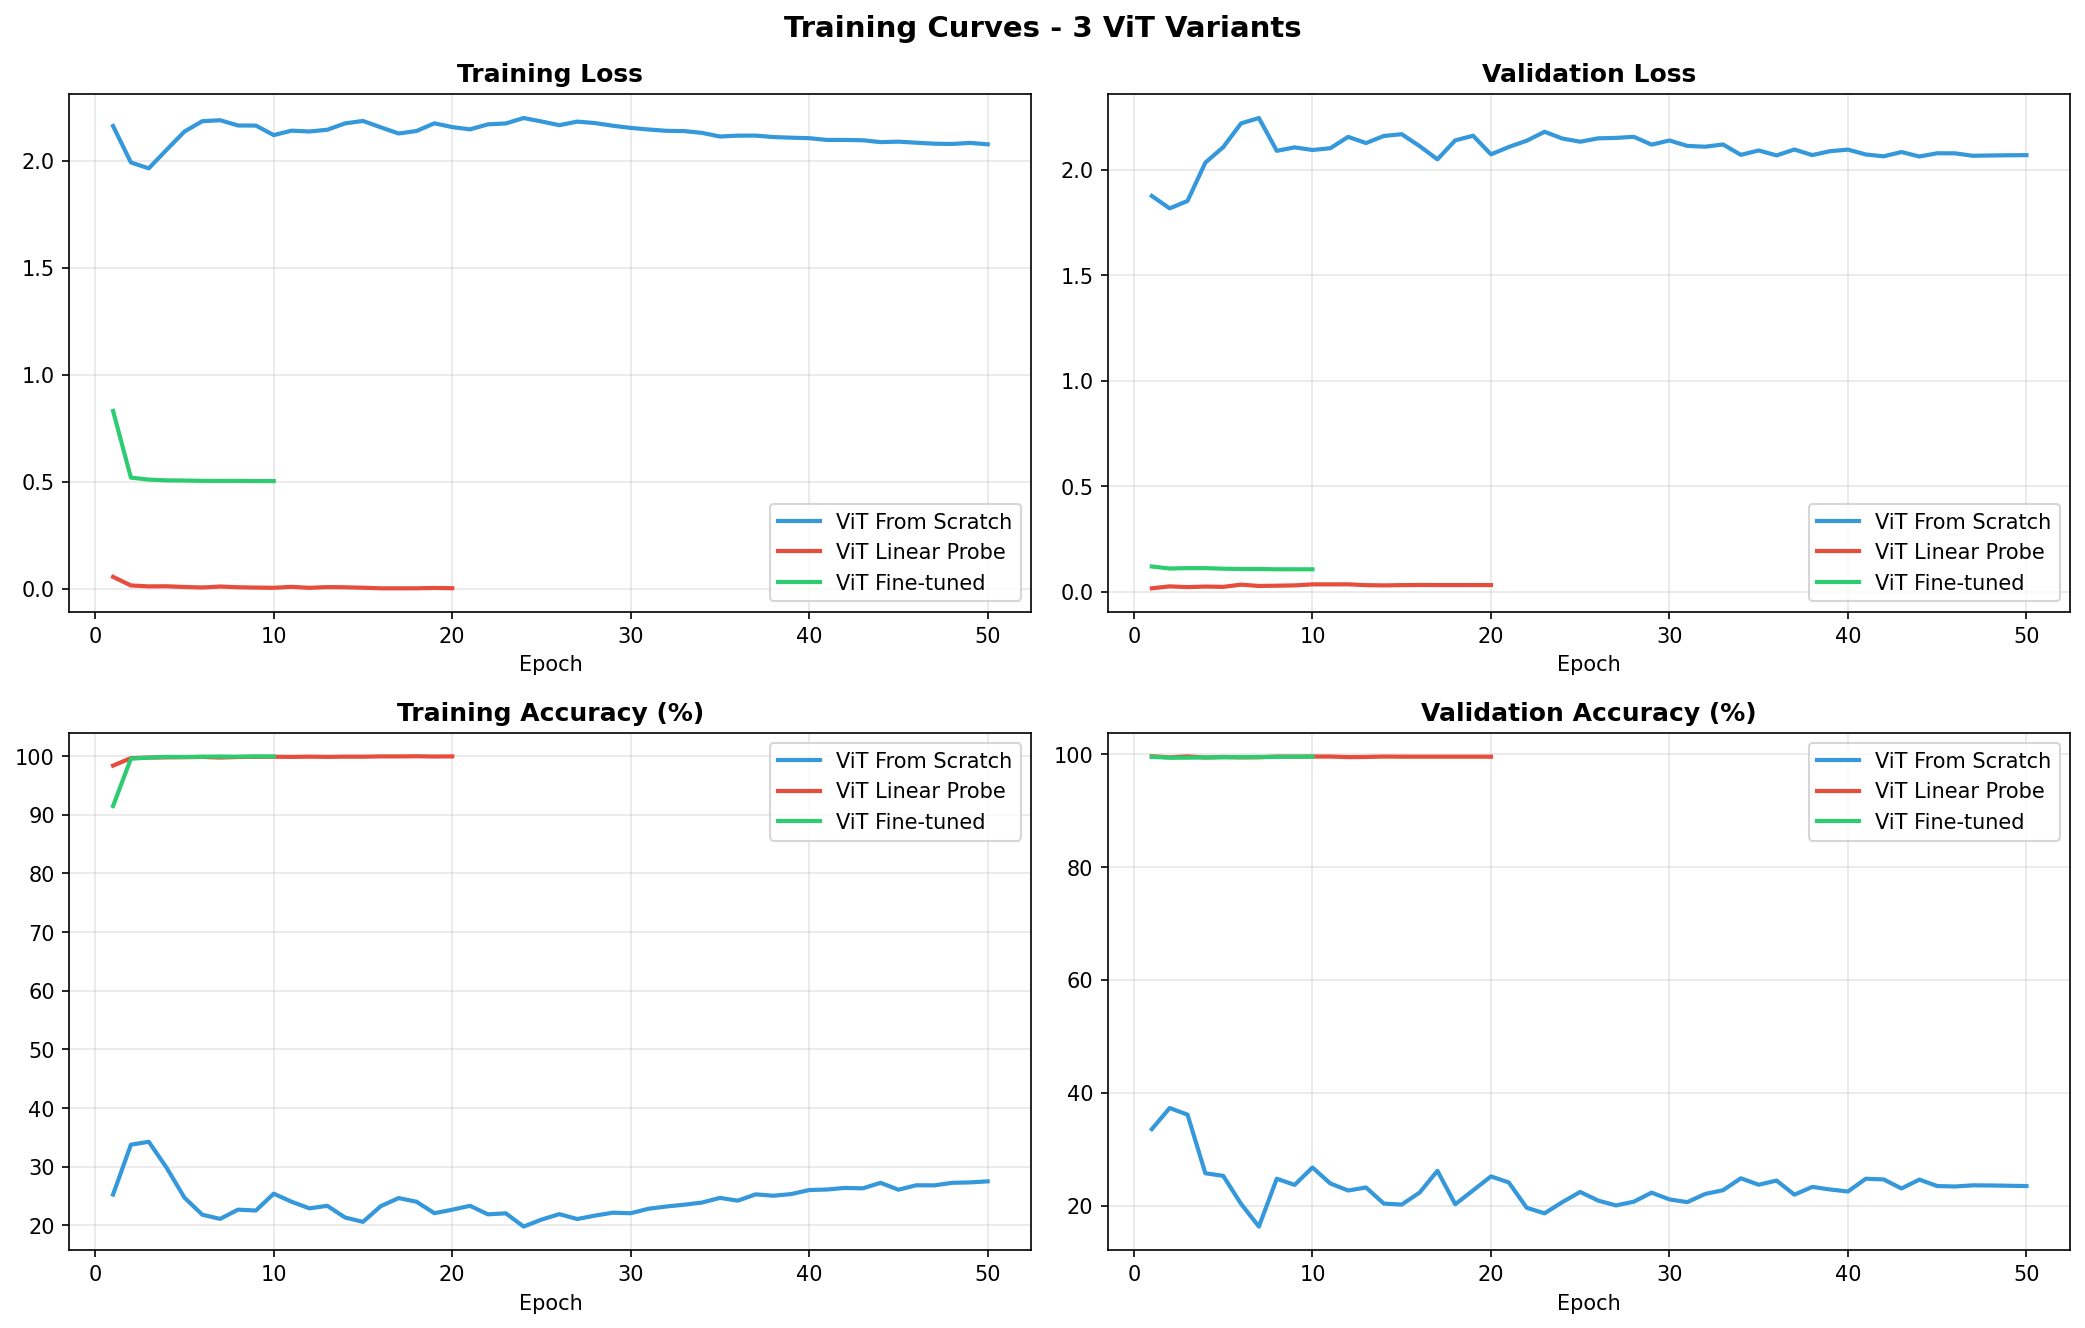
\includegraphics[width=0.72\textwidth]{figures/training_curves.png}
    \end{center}
    \vspace{-0.1cm}
    \scriptsize
    \xmark\ Scratch: peaked epoch 2 (37.30\%), degraded to 23.46\%.
    \cmark\ LP: 99.67\% (4.3 min).
    \cmark\ FT: 99.59\% (4.6 min).
\end{frame}

\begin{frame}
    \frametitle{Confusion Matrix Analysis}
    \begin{center}
        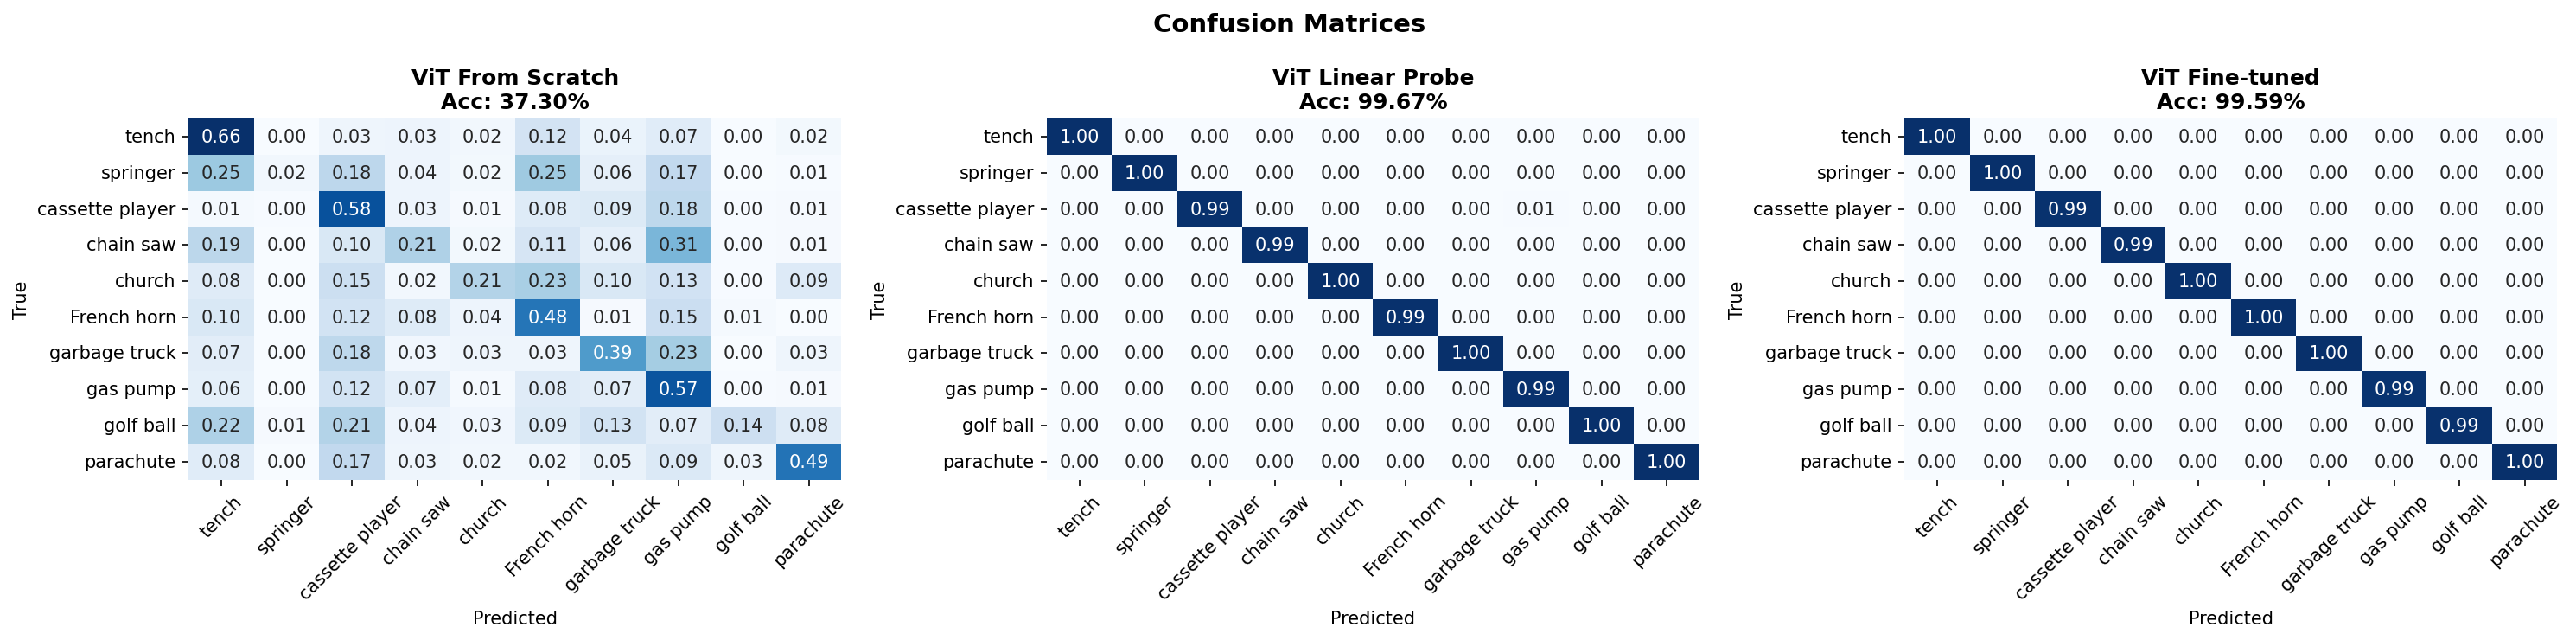
\includegraphics[width=0.95\textwidth]{figures/confusion_matrices.png}
    \end{center}
    \vspace{-0.1cm}
    \footnotesize
    \cmark\ Linear Probe \& Fine-Tuned: near-perfect diagonal. \xmark\ From Scratch: widespread confusion.
\end{frame}

\begin{frame}
    \frametitle{Per-Class Performance Analysis}
    \begin{center}
        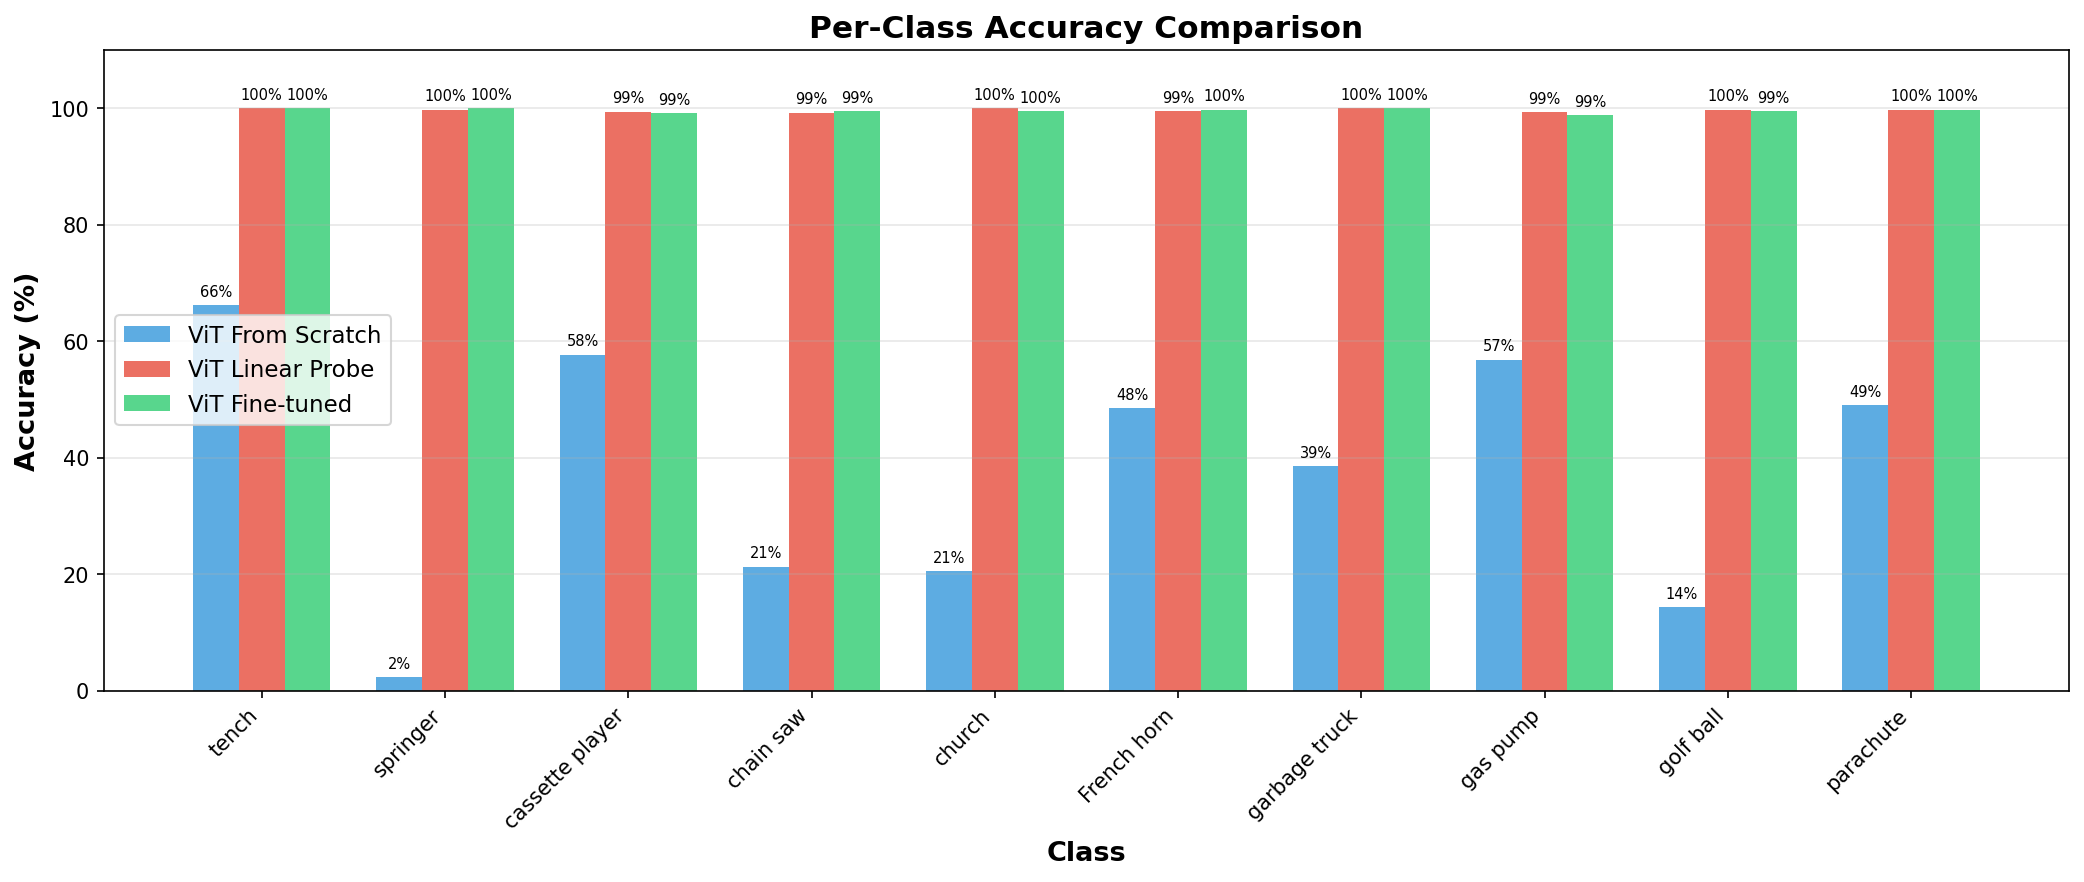
\includegraphics[width=0.85\textwidth]{figures/per_class_accuracy.png}
    \end{center}
    \vspace{-0.1cm}
    \footnotesize
    \cmark\ Pretrained models: high accuracy across all classes. \xmark\ From Scratch: inconsistent, some near zero.
\end{frame}

\begin{frame}
    \frametitle{All Metrics Comparison}
    \begin{center}
        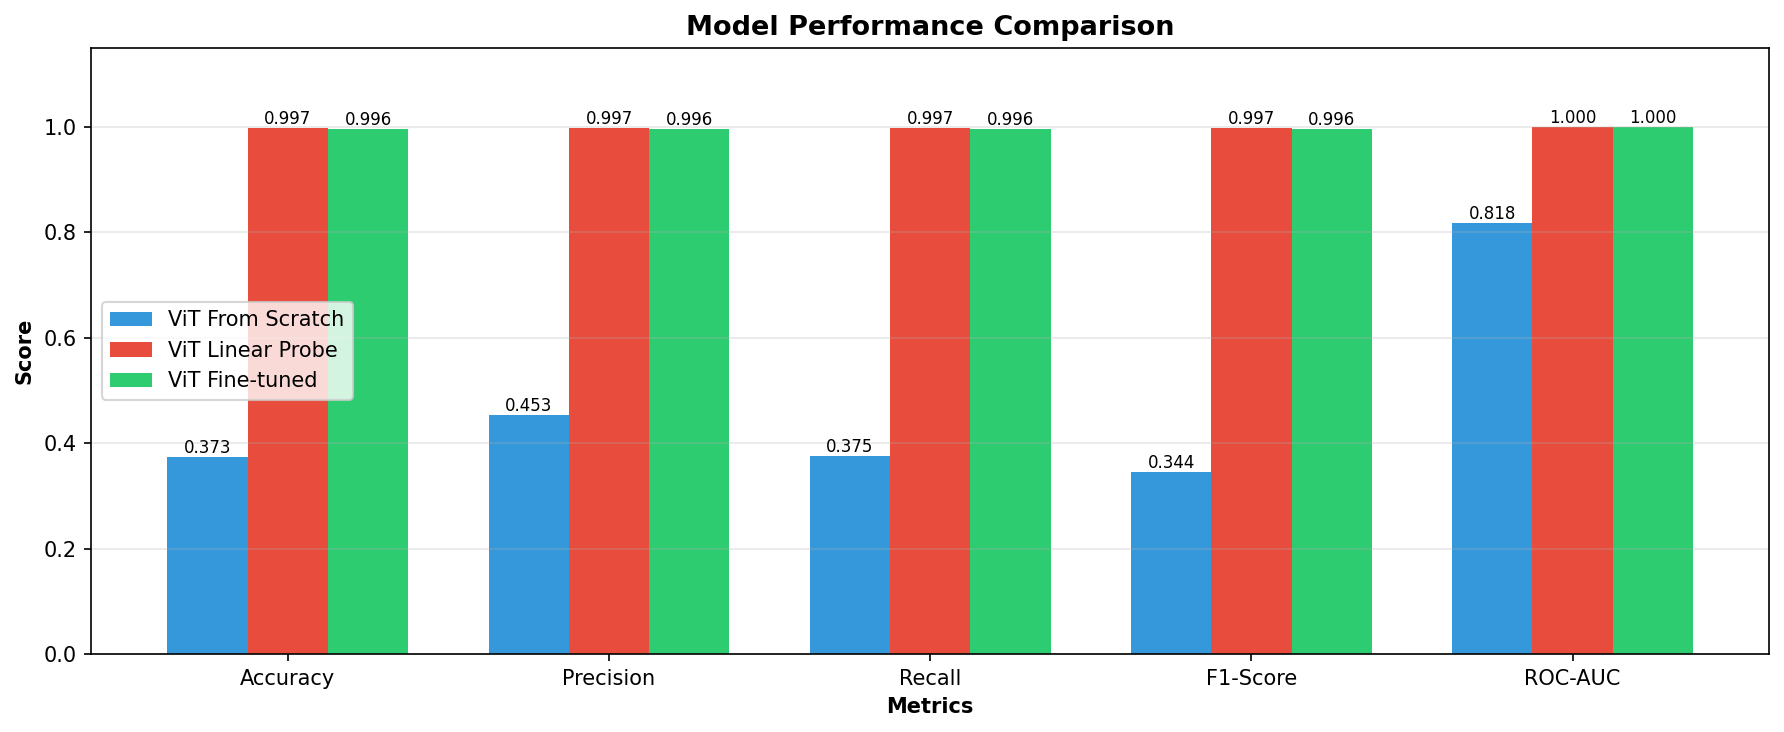
\includegraphics[width=0.68\textwidth]{figures/metrics_comparison.png}
    \end{center}
    \vspace{-0.1cm}
    \footnotesize
    \starmark\ \textbf{Linear Probe wins on ALL metrics.} Consistent: LP $>$ FT $>$ Scratch.
\end{frame}

\begin{frame}
    \frametitle{ROC Curve Analysis}
    \begin{center}
        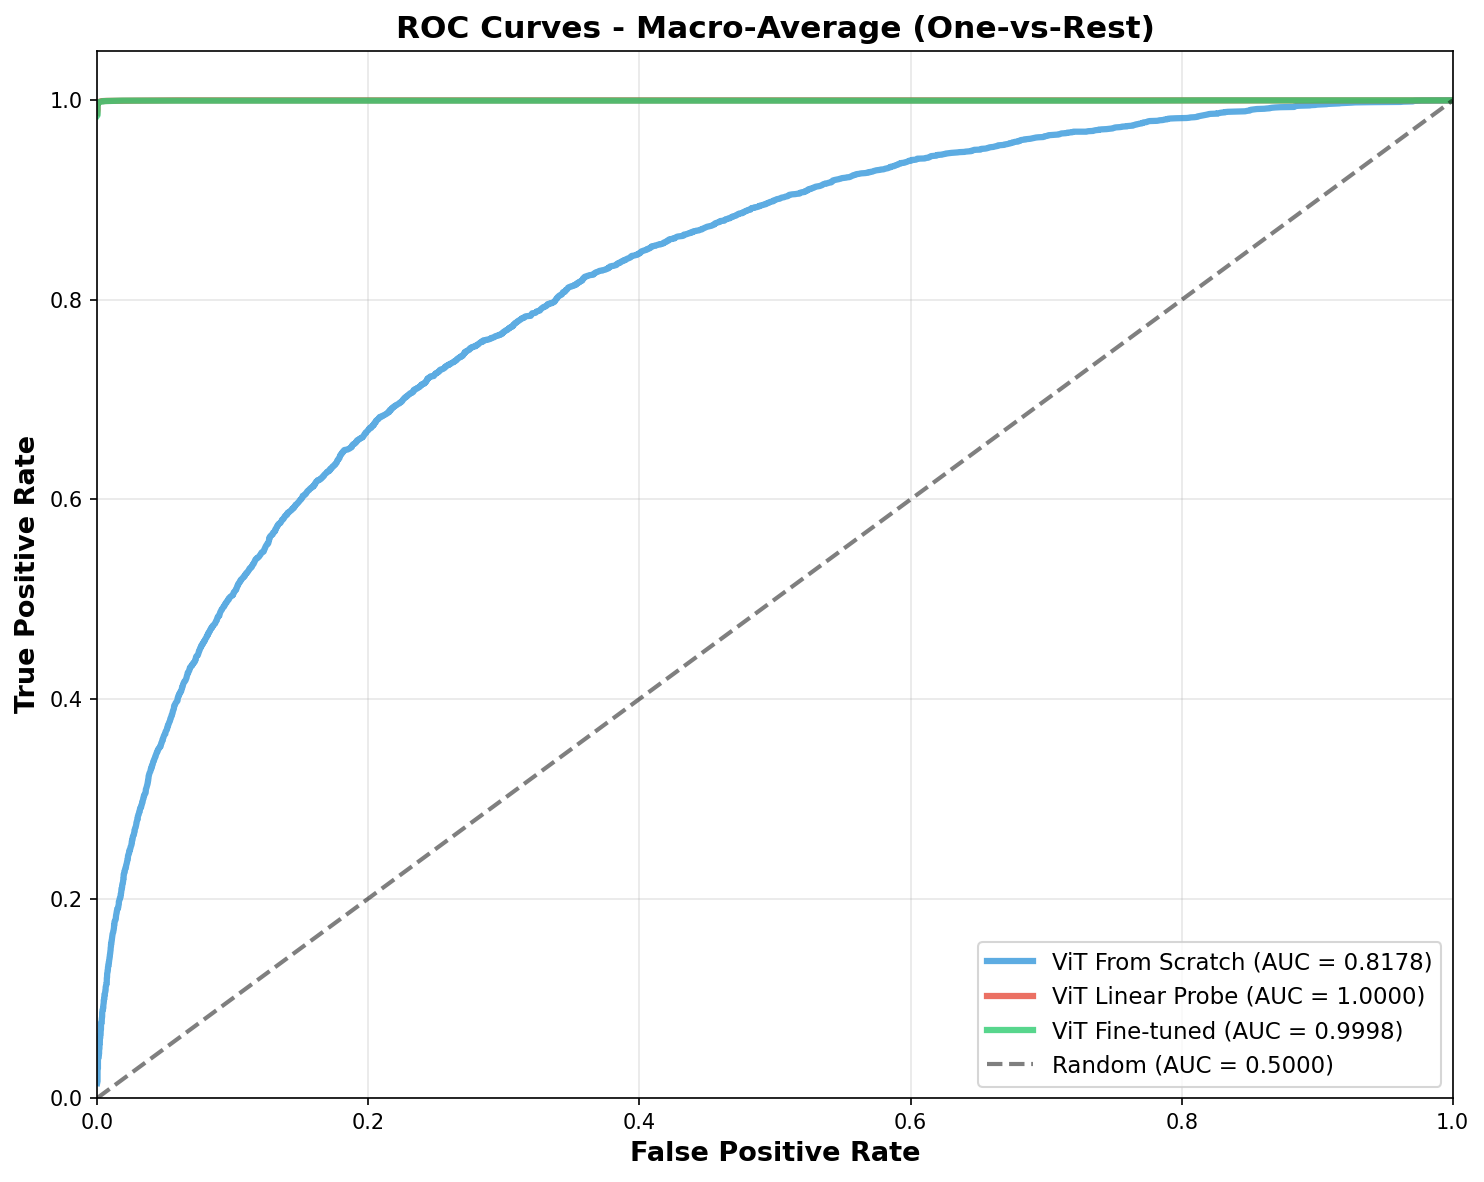
\includegraphics[width=0.55\textwidth]{figures/roc_curves.png}
    \end{center}
    \vspace{-0.1cm}
    \footnotesize
    \cmark\ Linear Probe: AUC = \textbf{1.0000} $\vert$ \cmark\ Fine-Tuned: 0.9998 $\vert$ \xmark\ From Scratch: 0.8176
\end{frame}

\begin{frame}
    \frametitle{Parameter Efficiency}
    \begin{center}
        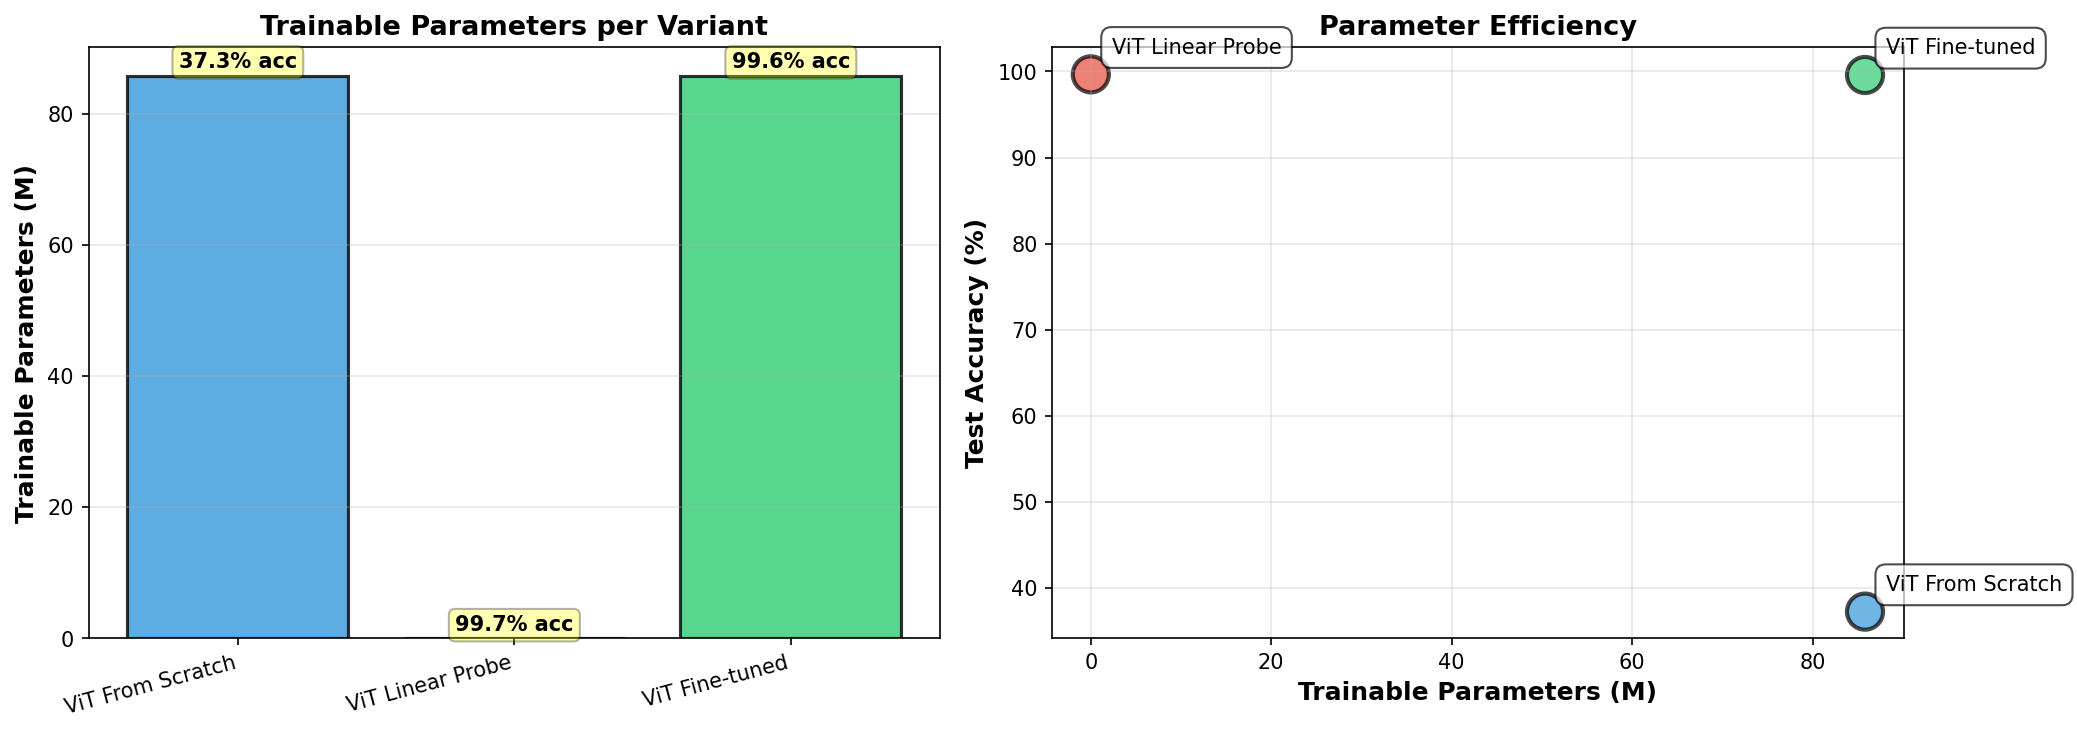
\includegraphics[width=0.75\textwidth]{figures/parameter_efficiency.png}
    \end{center}
    \vspace{-0.1cm}
    \begin{alertblock}{The Linear Probe Surprise}
        \footnotesize
        99.67\% with only \textbf{7,690 trainable params} (0.009\% of model)! Pretrained features are powerful even frozen.
    \end{alertblock}
\end{frame}

% ============================================================================
\section{Discussion}

\begin{frame}
    \frametitle{ViT Attention Maps: What the Model Sees}
    \begin{center}
        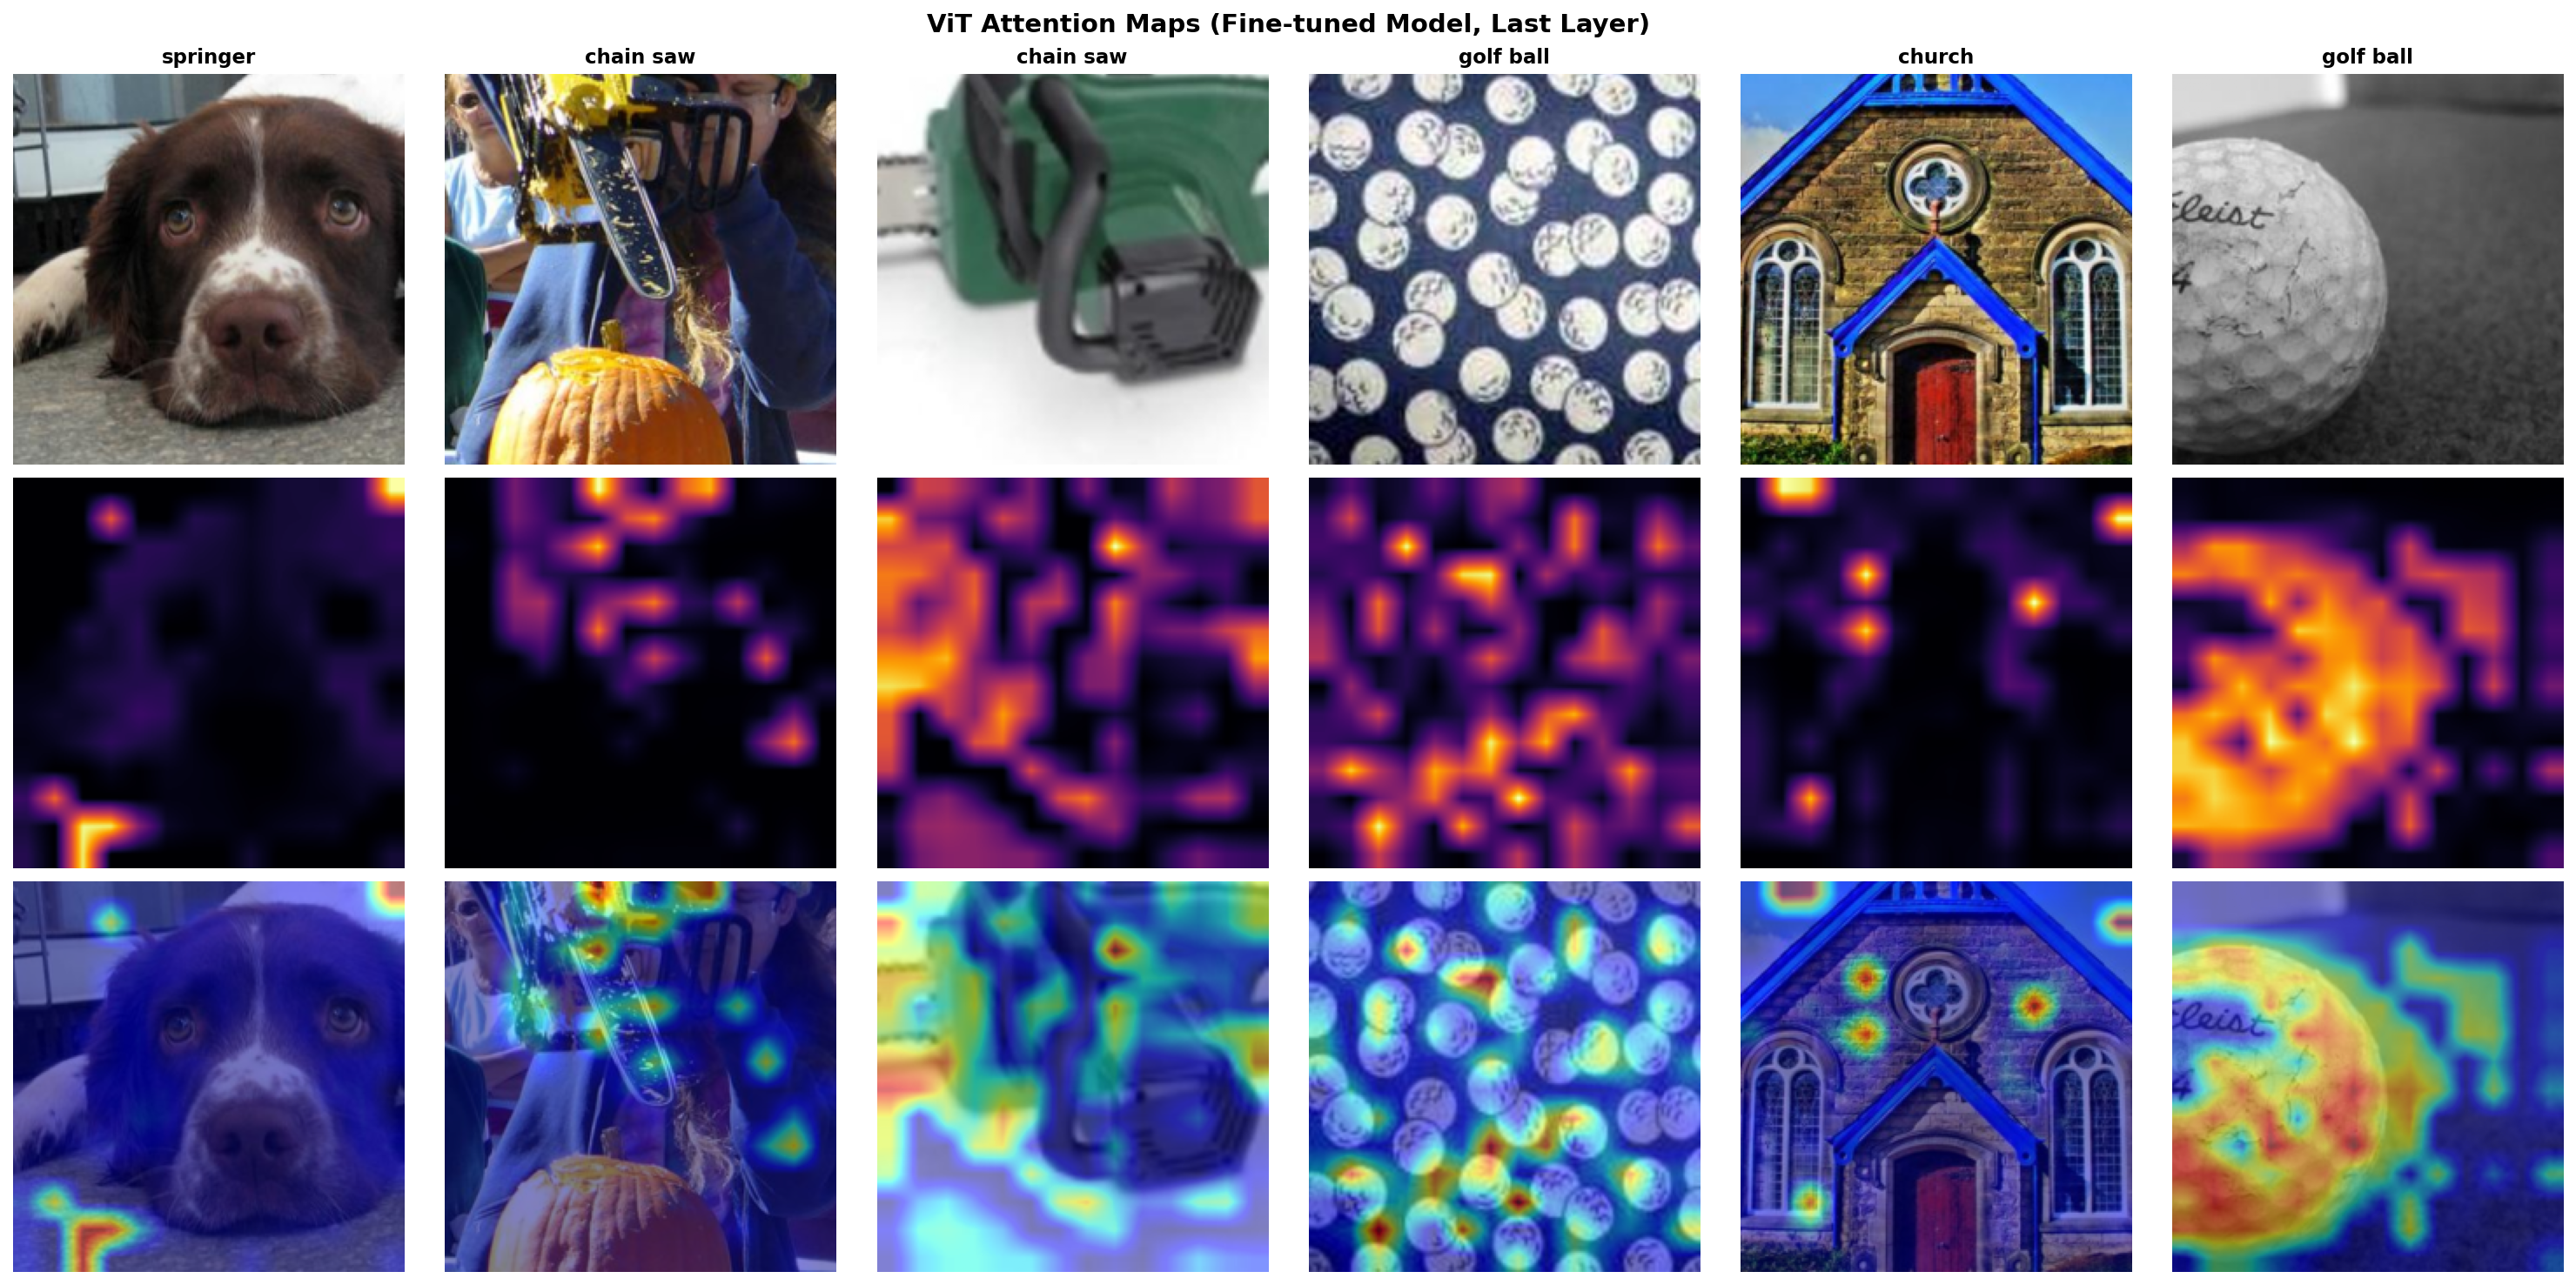
\includegraphics[width=0.82\textwidth]{figures/attention_maps.png}
    \end{center}
    \vspace{-0.1cm}
    \footnotesize
    Top: originals $\vert$ Middle: attention heatmaps $\vert$ Bottom: overlay. ViT focuses on the object.
\end{frame}

\begin{frame}
    \frametitle{Attention Evolution Across Layers}
    \begin{center}
        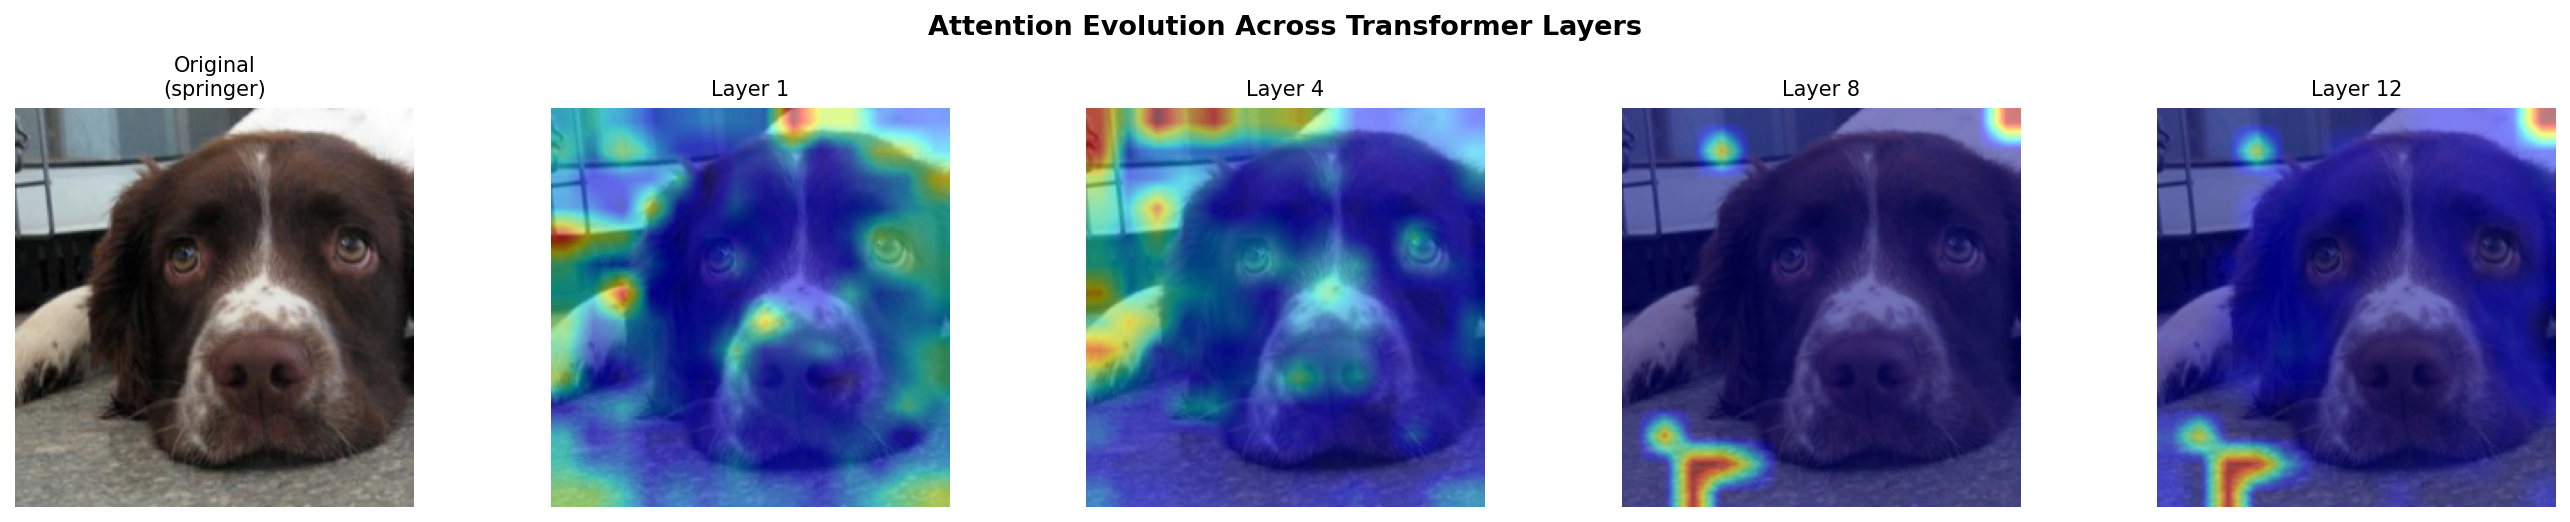
\includegraphics[width=0.88\textwidth]{figures/attention_layers.png}
    \end{center}
    \vspace{-0.1cm}
    \footnotesize
    \textbf{L1:} broad, diffuse $\rightarrow$ \textbf{L4:} object regions $\rightarrow$ \textbf{L8:} key features $\rightarrow$ \textbf{L12:} focused on discriminative parts.
\end{frame}

\begin{frame}
    \frametitle{Why Does Pretraining Matter So Much?}
    \footnotesize
    \textbf{Four Key Reasons:}
    \begin{enumerate}
        \item \textbf{No Inductive Bias} --- CNNs have locality (3$\times$3 filters) and translation equivariance. ViT has \textit{none}, must learn spatial relationships from scratch.

        \item \textbf{Data Hunger} --- Original ViT trained on 300M+ images. ImageNette has only $\sim$9,500 --- not enough!

        \item \textbf{Pretrained Features Transfer Well} --- ImageNet-21k provides rich representations. Even frozen features achieve 99.67\% (linear probe).

        \item \textbf{Fine-Tuning Adapts Efficiently} --- Small LR ($2 \times 10^{-5}$) + few epochs = pretrained knowledge + task adaptation.
    \end{enumerate}
\end{frame}

\begin{frame}
    \frametitle{Key Findings Summary}
    \small
    \begin{enumerate}
        \item \textbf{Linear Probe won:} 99.67\% accuracy --- beat Fine-Tuned (99.59\%)!
        \begin{itemize}
            \item 62.37 percentage points above from-scratch
            \item Frozen pretrained features (7,690 params) outperform full fine-tuning (85.8M params)
        \end{itemize}

        \item \textbf{ViT needs pretraining:} From-scratch fails on small datasets
        \begin{itemize}
            \item No inductive bias = must learn everything from data
            \item $\sim$9,500 images is not enough for 86M parameters
        \end{itemize}

        \item \textbf{Linear probe is shockingly strong:} 99.67\% with only 7,690 params
        \begin{itemize}
            \item 0.009\% of parameters, yet \textit{best} accuracy
        \end{itemize}

        \item \textbf{Attention maps provide interpretability}
        \begin{itemize}
            \item Can visualize what the model focuses on
            \item Not available in traditional CNN architectures
        \end{itemize}
    \end{enumerate}
\end{frame}

% ============================================================================
\section{Conclusion}

\begin{frame}
    \frametitle{Limitations \& Future Work}
    \small
    \textbf{Limitations:}
    \begin{itemize}
        \item Only tested on ImageNette (10 easy classes)
        \item Each strategy trained once (ideally multiple runs for statistics)
        \item Only ViT-Base tested (not ViT-Small or ViT-Large)
        \item Standard augmentation only (no RandAugment, MixUp, CutMix)
    \end{itemize}

    \vspace{0.15cm}

    \textbf{Future Work:}
    \begin{itemize}
        \item Harder datasets: ImageWoof (10 dog breeds), full ImageNet
        \item Model variants: ViT-Small, ViT-Large, DeiT
        \item Hybrid architectures: Swin Transformer, ConvNeXt
        \item Advanced fine-tuning: Layer-wise LR decay, progressive unfreezing
        \item Deployment: Pruning, quantization, knowledge distillation
    \end{itemize}
\end{frame}

\begin{frame}
    \frametitle{Conclusion}

    \begin{center}
        \Large
        \textbf{What We Proved:}

        \vspace{0.2cm}

        \normalsize
        Training strategy (pretrained features)

        \LARGE $>$

        \normalsize
        Training from scratch (same architecture, same data)

        \vspace{0.5cm}

        \begin{block}{}
            \centering
            \textbf{Pretraining is Everything for ViT!}\\
            \vspace{0.1cm}
            99.67\% linear probe vs 37.30\% from scratch $\vert$ 7,690 vs 85.8M params
        \end{block}

        \vspace{0.15cm}

        \small
        \textbf{Evolution:} CNN $\rightarrow$ ResNet (skip connections) $\rightarrow$ \textbf{ViT (pretraining + attention)}

        \vspace{0.3cm}

        {\Huge Thank You!}\\[0.15cm]
        {\Large Questions \& Discussion}\\[0.15cm]
        \footnotesize
        \textbf{Junjie} $\vert$ MSCS 2203 $\vert$ Computer Science $\vert$ March 2026
    \end{center}
\end{frame}

\end{document}
